\chapter{CPU, Scheduling, and OS Services}

\section{Measurement overhead}
In this part, we measure the overhead of reading time(read processor cycle counter) and the overhead of using a loop to measure many iterations of an operation. We will use these data to make other experiments more accurate by removing the overhead.

\paragraph{Methodology}
According to the hint, we googled rdtsc instruction and find useful helper functions rdtsc()\cite{rdtsc}, written in inline assembly form that return processor cycle count. 

In order to record the overhead of reading time, we call rdtsc() twice and subtract them. To measure the overhead of using a loop, we apply this method
\lstinputlisting[language=C]{hello.c}
We run it many times, and get the overhead by (end - start) / loops.

\paragraph{Predictions}
As for reading time, I guess the overhead of software is 8 cycles which I get from the inline assembly code. For the hardware layer, I guess it is 9 cycles to perform read, binary operation, write. So total 17 cycles for reading time; 

As for iterations of an operation, I guess software takes 3 cycles to do branch and increment and hardware takes 1 or 2 cycles as overhead, so it is about 5 cycles for iterations.

\paragraph{Results}
We present our measure results.

\begin{center}
\begin{tabular}{| p{2cm} | p{3cm} | p{3cm} | p{2cm} | p{3cm} | p{1cm} }
Operation  & Base Hardware Performance  & Estimated Software Overhead  & Predicted Time  & Measured Time  & Std  \\
\hline
Reading time & 9 cycles& 8 cycles& 17 cycles& 19.51327 cycles  & 1.9087  \\
Using a loop  & 2 cycles& 3 cycles& 5 cycles& 5.726476 cycles & 0.1728 \\
\end{tabular}
\end{center}

\paragraph{Discussion}
My prediction is pretty successful, very close to the measure value. Because we adopted low-overhead mechanism to measure operations and these operations are visible to use, we could follow and predict all the instructions they perform. So our prediction and methodology could get this result. 

\section{Procedure call overhead}
In this part, we measure the overhead of Procedure call. 

\paragraph{Methodology}
In order to get accurate result, we have to tell compiler not to inline the procedure call. So We use this attribute ((noinline)) to tell gcc not to inline procedure call and I turn off OPTIMIZE.

We did not process the arguments in procedure call. We iterate about 100000 times, I record the counter before the loop and record it again after the loop, then remove the iteration overhead.

\paragraph{Predictions}
We predicte when adding more arguments to procedure call, the cycle count should increase linearly. Because we should push each argument to the stack. Besides, procedure call will maintain stack pointers, and instruction like call and ret. When there are no arguments, the cycle should be about 6 cycles, 4 cycles for call, ret and maintain stack pointers and 2 cycles for hardware. When adding one more arguments, we assume hardware and software both add 1 cycles.


\paragraph{Results}
We present our measure results(unit : cycle).

\begin{center}
\begin{tabular}{l*{6}{c}r}
Args              & Hardware  & Software  & Overall  & Measured  & Remove overhead & Std\\
\hline
0 args & 2 & 4 & 6 & 7.1 & 2.1 & 0.16788\\
1 args & 3 & 5 & 8 & 7.3  & 2.3 & 0.19758 \\
2 args & 4 & 6 & 10 & 7.7 & 2.7 & 0.17281 \\
3 args & 5 & 7 & 12 & 8.6 & 3.6 & 0. 21230  \\
4 args & 6 & 8 & 14 & 9.3 & 4.3 & 0. 26652 \\
5 args & 7 & 9 & 16 & 10.0 & 5.0 & 0.17272 \\
6 args & 8 & 10 & 18 & 10.9 & 5.9 & 0.20281 \\
7 args & 9 & 11 & 20 & 13.1 & 8.1 & 0.22101 \\
\end{tabular}
\end{center}

\begin{figure}[htbp] %  figure placement: here, top, bottom, or page
   \centering
   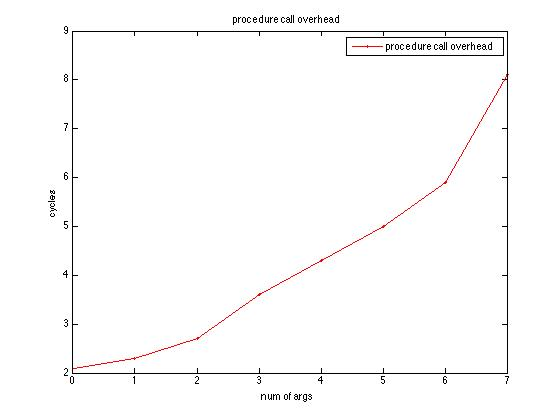
\includegraphics[width=5in]{./pics/pcall.jpg} 
   \caption{procedure call overhead}
   \label{fig:procedure call overhead}
\end{figure}

\paragraph{Discussion}
The measurement statistics is a little strange. Like we have predicted, the overhead for a procedure call scales about linearly with the number of arguments passed in; However, the cycles procedure calls take are less than we have predicted. 

So I tried another methodology. In a loop, first I record the counter, then do procedure call and record again. When calculating, I remove the overhead of counter reading time. But I still get similar results.

I have guessed that compiler may use registers to store parameter in the loop so as to reduce many memory operations. So I look at assembly code but it is pretty regular stack operation.

With the increasing of iteration time, the average cycles decrease a lot. There may be some mechanism like cache in the hardware.

\paragraph{Question} What is the increment overhead of an argument? The increment overhead is about 1 cycle per  argument, pushing parameters to stack.

\section{System call overhead}
In this part, we measure the overhead of System call. There are more than 100 systems in Mac OS and Linux like exit, fork, open and getpid. And the overhead varies a lot. For example, System call like fork will use more cycles than getpid. Because fork will creates a new process by duplicating the calling process which will use much more resources than getpid. So we aim to choose the one that use fewer CPU cycles. The minimal cost can be emulated by measuring the cost of getpid() or getppid().

\paragraph{Methodology}
Because in my operating system getpid() will cache the result. So we use a trick here. In each iteration, we fork a child process, and call getpid() in child process and then reap this child process. So every iteration we actually call getpid() in a bread-new  process, as a result we will never call getpid() on a cached one. So we solved this problem.

As before, we iterate about 100000 times, record the time before getpid() and after getpid(), then calculate the average cycles.

\paragraph{Predictions}
As for hardware, it may take 200 cycles to deal with registers. As for software, it is hard to estimate.  I know the operations including save current state to memory, trap into kernel, then kernel provide service and finally restore previous state. I measure it about 10000 cycles.

\paragraph{Results}
We present our measure results.

\begin{center}
\begin{tabular}{| p{2cm} | p{3cm} | p{3cm} | p{2.5cm} | p{2.5cm} | p{2cm}}
System call  & Base Hardware Performance  & Estimated Software Overhead  & Predicted Time  & Measured Time  & Std \\
\hline
getpid() & 200 cycles& 10000 cycles& 10200 cycles& 43020 cycles & 1702\\
\end{tabular}
\end{center}

\paragraph{Discussion}
Our estimates were lower than the measured result. That is to say, the overhead of user and kernel mode switch is more than we have imagined. So, caching some system call results may be a good idea. Because some stupid system call benchmark will repeatedly call getpid ().

\paragraph{Question} How does it compare to the cost of a procedure call? The cost of a system call is much larger than that of a procedure call. Because a system call involves switch between user mode and kernel mode. Furthermore, kernel will provide service to the caller and sometimes will have I/O operations.

\section{Task creation time}
In this part, we measure task creation time, measure the time to create and run both a process and a kernel thread.

\paragraph{Methodology}
For process, we use fork() to create a new process.  Each iteration we record time before fork(). Then there is a problem : Who executes first after fork(), parent or the child? In general, nothing can be said about the relative order of their execution. So we can not record time immediately after fork(). Here is our trick : in child process, we simply exit(); But in parent process, we use wait(NULL) and then record time. So after fork(), first parent process will give CPU to child process, then child process exit and kernel give CPU to parent process again. So there are two context switches. Then we subtract the two context switch overheads and get the final results. We run there procedure many times and get the average.

Things are quiet similar for kernel thread. We use pthread to create a task. Whenever we create a new thread, in the thread function we use pthread\_exit() to kill thread immediately, which will make measurement accurate.

\paragraph{Predictions}
It is difficult to predict accurately. What I am quiet sure is that creating a thread kernel is much more cheaper than creating a process. Because threads share many resources like file descriptors.

THOMAS E. ANDERSON in 1991 report it takes 11300 microseconds to fork process and 948 microseconds to create thread. \cite{task} In 1991, the CPU frequency of Intel 80486SX is 20MHz. Based on CPU frequency at that time, which are about 200000 cycles to fork process and 20000 cycles to create thread. So I do the following predictions.

For process, I guess the hardware overhead are 10000 cycles, and the software overhead is 190000 cycles.
For thread, I guess the hardware overhead are 1000 cycles, and the software overhead is 19000 cycles.

\paragraph{Results}
We present our measure results.

\begin{center}
\begin{tabular}{| p{2cm} | p{3cm} | p{3cm} | p{2.5cm} | p{2.5cm} | p{2cm} }
Task creation  & Base Hardware Performance  & Estimated Software Overhead  & Predicted Time  & Measured Time  & Std \\
\hline
process & 10000 cycles& 190000 cycles& 200000 cycles& 311751  cycles & 11321 \\
kernel thread    & 1000 cycles& 19000 cycles& 20000 cycles& 16509 cycles & 827\\
\end{tabular}
\end{center}

\paragraph{Discussion}
First, the cost of creating a process is much more expensive than a thread as the data indicated. Because thread is a light process that share many resources so it use fewer CPU cycles.

\paragraph{Question} How do they compare?
The cost of creating a new process is expensive. Each process has its own address space. Even with COW, there are still many memory copy operation and other overheads. Compared with process, kernel thread can share process resources and can be used in many situations. For example, in a web server, there are many clients and it is impossible to respond to so many clients using process creation model.

\section{Context switch time}
In this part, we measure the time to context switch from one process to another, and from one kernel thread to another.

\paragraph{Methodology}
As the hint indicated, blocking pipe will force context switch and we tried, it did do context switch so we use blocked pipe to perform context switch.

For process, we first record the time before read pipe, because read will block so it will switch to child process. Then we record the end time and write end time to pipe. So when parent process resume, parent process can collect the end time and do the calculation; Besides, we use wait() to reap resources.

For thread, we perform similar operations. After pthread\_create(), we record start time and use read to block pipe. At thread function we record the end time and write this value to pipe. So main thread could collect data and print the statistics.

At the end of each iteration, we all reap the resource in order to get accurate results. When there are many resources that are not reaped, our machine may run slower than usual.

\paragraph{Predictions}
What I am sure is that process context switch is much more expensive than thread context switch.

For process context switch, I think hardware cycles are 20000 cycles and software are 5000 cycles.

For thread context switch, I think hard cycles are 2000 cycles and software are 500 cycles.

\paragraph{Results}
We present our measure results.

\begin{center}
\begin{tabular}{| p{2cm} | p{3cm} | p{3cm} | p{2.5cm} | p{2.5cm} | p{2cm} }
Context switch              & Base Hardware Performance  & Estimated Software Overhead  & Predicted Time  & Measured Time & Std  \\
\hline
process & 20000 cycles& 5000 cycles& 25000cycles & 133221 cycles & 3428 \\
kernel thread    & 2000 cycles& 500 cycles& 2500 cycles& 9752 cycles & 439 \\
\end{tabular}
\end{center}

\paragraph{Discussion}
We predict well on the scale of process context switch and thread context switch. A process contains much more information than a kernel thread, so it is expensive of course just like previous experiments on creation time overhead.

The cost of process context switch is as expensive as fork a new process and so as a kernel thread. So context switch is very important to go deep into. How to reduce the overhead of context switch is of great significance.

\paragraph{Question} How do they compare?
In my experiment, kernel threads are approximately 14 times faster in performing a context switch than processes. So in some applications like web server, threads are much more cheaper than processes and recommended.